
  \chapter{Schemat działania projektu}
  
    \section{Założenia}

    Zostały zdefiniowane ogólne założenia dotyczące każdego z elementów, których spełnienie definiuje kryterium sukcesu.
    
    \begin{itemize}
        \item    System składa się z trzech głównych elementów, połączonych ze sobą:
            \begin{itemize}
                \item urządzenia wykonawczego,
                \item brokera MQTT,
                \item aplikacji dostępowej.
            \end{itemize}
            
        \item     Komunikacja pomiędzy częściami składowymi odbywa się z poprzez sieć bezprzewodową wykonaną w technologii WiFi z wykorzystaniem protokołu MQTT.
        \item     Urządzenie wykonawcze ma zadawać napięcia na silnik prądu stałego w taki sposób, aby uzyskać parametry jak najbardziej zbliżone do zadanych przez aplikację dostępową.   
        \item    Aplikacja dostępowa ma za zadanie stanowić prosty i przejrzysty interfejs do sterowania urządzeniem. Umożliwia ona:
    
            \begin{itemize}
                \item zadawania prędkości obrotowej silnika,
                \item odczytu aktualnej prędkości silnika,
                \item zmiany nastaw regulatora PID,
                \item odczytu napięcia zasilania urządzenia,
                \item odczytu wypełnienia sygnału PWM.
            \end{itemize}
            
        \item    Broker MQTT on za zadanie być lekkim i szybkim pośrednikiem w komunikacji między aplikacją dostępową, a urządzeniem wykonawczym.
    \end{itemize}
 
 
    \section{Architektura systemowa}
        Projekt opiera się o współpracę trzech kluczowych elementów ciągle komunikujących się ze sobą. Komponenty wchodzące w skład systemu zostały umieszczone na rysunku \ref{fig:system}.
        
        \begin{figure}[ht]
          \centering
          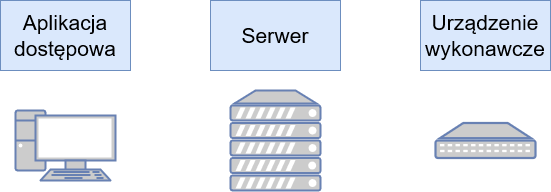
\includegraphics[width=1\textwidth]{img/system.png}
          \caption{Elementy systemu}
          \label{fig:system}
        \end{figure}


        \subsection{Aplikacja dostępowa}
            W celu komfortowej obsługi sterownika silnika, została stworzona aplikacja dostępowa w języku C++, która będzie komunikowała się w protokole MQTT. W tym celu wykorzystano otwarto źródłową wersję narzędzia programistycznego jakim jest QT \cite{qt}. Biblioteki QT posiadają dobrze zdefiniowane warstwy abstrakcji oraz bardzo wylewną dokumentację, co sprawia że tworzenie zaawansowanych, przenośnych aplikacji okienkowych jest niezwykle łatwe i przyjemne.
        
        \subsection{Urządzenie wykonawcze}
            Urządzenie końcowe jest dedykowanym rozwiązaniem przygotowanym specjalnie na poczet tego projektu. Bazuje ono na nowoczesnym SoC z rodziny ESP32, który łączy się z brokerem MQTT. Odbierane z niego dane wykorzystane są w procesie sterowania silnikiem. Poza odczytem informacji z brokera, urządzenie publikuje również aktualny stan silnika.
        
        \subsection{Serwer}
            Ostatnim elementem projektu jest Broker MQTT. Jego zadaniem jest bycie łącznikiem pomiędzy urządzeniami. Pozwala on na łatwe subskrybowanie jak i publikowanie informacji. Ta rola przypadła dla otwarto źródłowego brokera Mosquitto wydanego przez fundację Eclipse \cite{mosquitto}. Jest to jeden z popularniejszych programów tego typu, a zawdzięcza to małym wymaganiom sprzętowym, skalowalności oraz
            dostępności na wielu architekturach sprzętowych. Co więcej, w celu wdrożenia
            przenośności projektu, oprogramowanie to zostało poddane konteneryzacji,
            dzięki czemu można łatwo transportować go i uruchamiać na innych komputerach wraz z całą konfiguracją przy użyciu ekosystemu Docker \cite{docker}.
            
 
    \section{Wymiana informacji}
        
        W protokole MQTT kluczowy aspekt mają tematy, z angielskiego "Topics". Pozwalają one na wymianę i porządkowanie informacji. Każda nadawana wiadomość jest kierowana do konkretnego tematu na brokerze. W celu odbioru wiadomości niezbędna jest subskrypcja danego tematu.

    \subsection{Wykorzystywane tematy}
        Tematy tworzone i zarządzane przez aplikację okienkową to:
    
        \begin{itemize}
          \item kp - Wartość członu proporcjonalnego. Parametr sterujący pracą regulatora PID,
          \item ki - Wartość członu całkującego. Parametr sterujący pracą regulatora PID,
          \item kd - Wartość członu różniczkującego. Parametr sterujący pracą regulatora PID, 
          \item setpoint - Wartość zadana dla regulatora. Wyrażona w obrotach na minutę. 
        \end{itemize}
    
        Należy zauważyć że są to tylko i wyłącznie wartości zarządzające pracą regulatora PID. Dzięki udostępnieniu ich poza obszar programu istnieje możliwość dynamicznej zmiany parametrów regulatora, co sprawia że nawet osoba nie mająca dużego doświadczenia z regulatorami PID potrafi empirycznie wyznaczyć zadowalające wartości. 
        
        \vspace{1em} 
        Poza tematami utworzonymi przez aplikację dostępową, potrzebne są jeszcze trzy dodatkowe tematy:
    
        \begin{itemize}
          \item rpm - ilość obrotów odczytana z silnika przy pomocy enkodera. Wyrażona w obrotach na minutę. Służy jedynie w celach kontrolnych. Daje możliwość zorientować się z jaką prędkością obraca się silnik w rzeczywistości i porównać wynik z wartością zadaną.
          
          \item pwm\_duty - wartość wypełnienia PWM, wyrażona w procentach. Obrazuje stopień wykorzystania dostępnej mocy silnika.
          
          \item voltage - Napięcie zasilania urządzenia. 
          
          %Według specyfikacji L298 napięcie dostarczane do silników jest niższe o 1.8V - 3.2V w zależności od obciążenia. \cite{mostek}
        \end{itemize}
        
        Obaj klienci brokera MQTT subskrybują nawzajem swoje tematy. Schemat wymiany danych został przedstawiony na rysunku \ref{data_transmision}. Obrazuje on sposób komunikacji i zależności.
        
    
        \begin{figure}[ht]
          \centering
          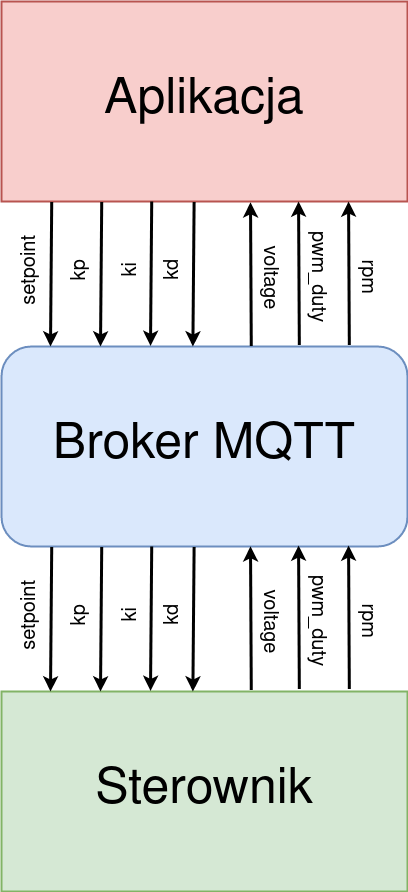
\includegraphics[height=0.8\textheight]{img/dane.png}
          \caption{Schemat wymiany danych w systemie}
          \label{data_transmision}
        \end{figure}